\definecolor{corecolor}{RGB}{0,50,255}
\definecolor{chipcolor}{RGB}{200,200,200}
\definecolor{gpucolor}{RGB}{118,185,0}
\definecolor{ramcolor}{RGB}{179,89,0}
\definecolor{nodecolor}{RGB}{120,120,120}

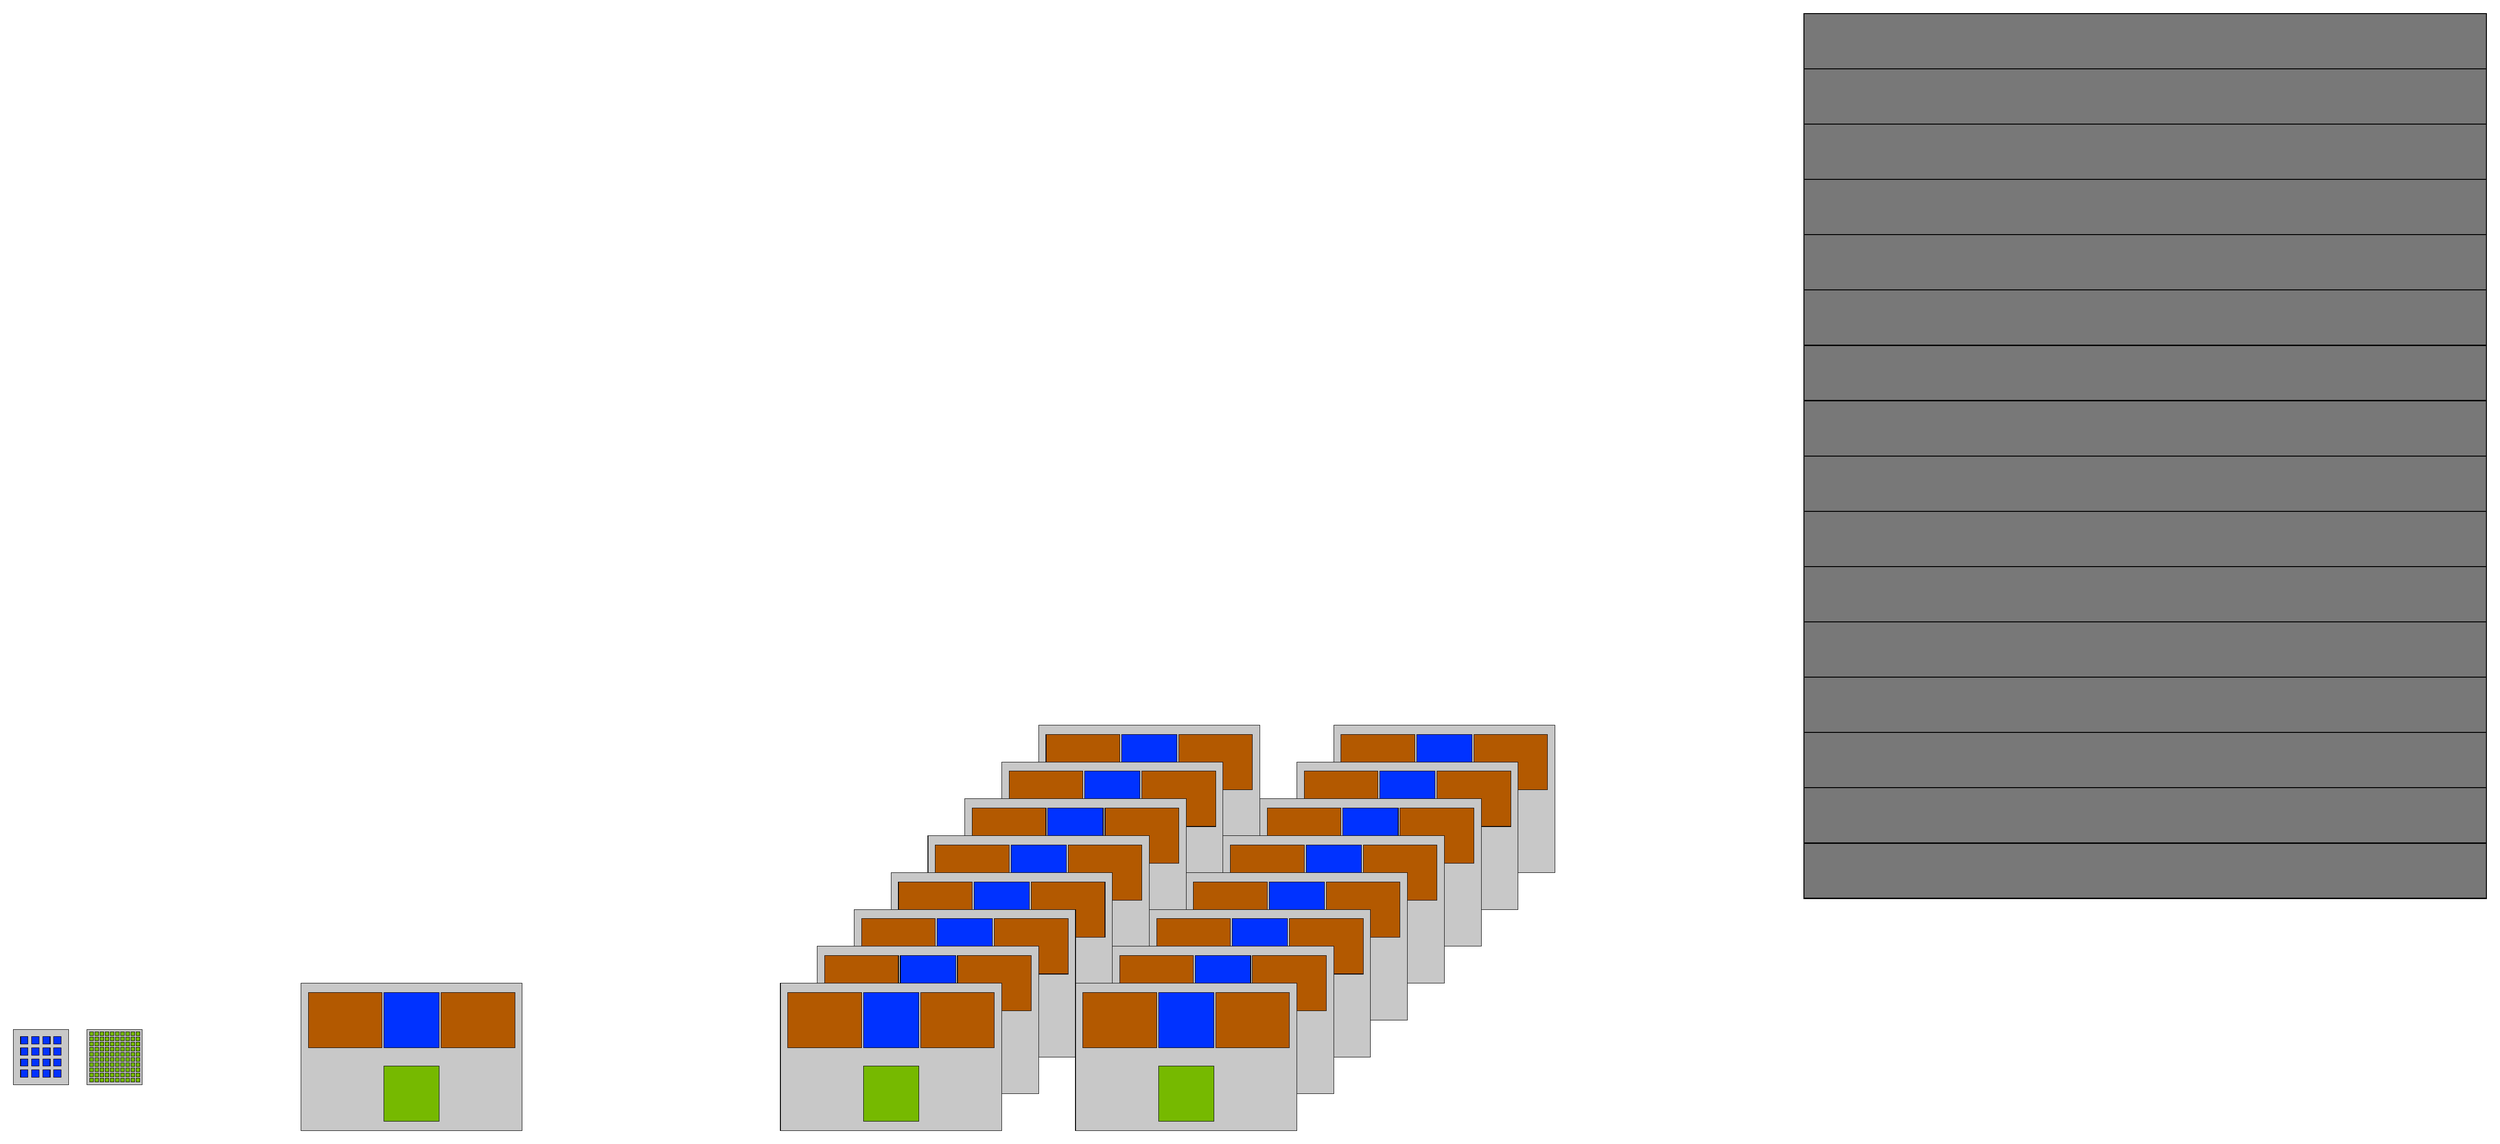
\begin{tikzpicture}
% First ethe chips
\begin{scope}[shift={(-3,0)}]
\begin{scope}[]
\node (rect) at (.95,.95) [fill=chipcolor,draw,minimum width=1.5cm,minimum height=1.5cm] () {};

\foreach \i in {0,1,2,3}{
	\foreach \j in {0,1,2,3}{
		\node (rect) at (\i*.3+.5,\j*.3+.5) [fill=corecolor,draw, minimum width=.2cm,minimum height=.2cm,inner sep=0pt] () {};
	}
}
\end{scope}

\begin{scope}[shift={(2,0)}]
\node (rect) at (.95,.95) [fill=chipcolor,draw,minimum width=1.5cm,minimum height=1.5cm] () {};

\foreach \i in {0,1,2,3,...,9}{
	\foreach \j in {0,1,2,3,...,9}{
		\node (rect) at (\i*.14+.32,\j*.14+.32) [fill=gpucolor,draw, minimum width=.1cm,minimum height=.1cm,inner sep=0pt] () {};
	}
}
\end{scope}
\end{scope}

% Then the Compute card 
\begin{scope}[shift={(8,0.95)}]
% Card base 
\node (rect) at (0,0) [fill=chipcolor,draw,minimum width=6cm, minimum height=4cm,inner sep=0pt] () {};
% CPU 
\node (rect) at (0,1) [fill=corecolor,draw,minimum width=1.5cm, minimum height=1.5cm,inner sep=0pt] () {};
% GPU 
\node (rect) at (0,-1) [fill=gpucolor,draw,minimum width=1.5cm, minimum height=1.5cm,inner sep=0pt] () {};
% RAM 
\node (rect) at (-1.8,1) [fill=ramcolor,draw,minimum width=2cm, minimum height=1.5cm,inner sep=0pt] () {};
\node (rect) at (1.8,1) [fill=ramcolor,draw,minimum width=2cm, minimum height=1.5cm,inner sep=0pt] () {};
\end{scope}

\begin{scope}[shift={(21,0.95)}]
% Add the base of the card 
%\node[fill=nodecolor,trapezium, draw, minimum width=3cm,
%trapezium left angle=46, trapezium right angle=-46,draw,
%minimum width=6cm,minimum height=9cm,inner sep=0] at (7,2) {A};

% Card base copied n times 
\foreach \i in {7,...,0}{
\foreach \j in {1}{
\begin{scope}[shift={(\i,\i)}]
\node (rect) at (0,0) [fill=chipcolor,draw,minimum width=6cm, minimum height=4cm,inner sep=0pt] () {};
\node (rect) at (0,1) [fill=corecolor,draw,minimum width=1.5cm, minimum height=1.5cm,inner sep=0pt] () {};
\node (rect) at (0,-1) [fill=gpucolor,draw,minimum width=1.5cm, minimum height=1.5cm,inner sep=0pt] () {};
\node (rect) at (-1.8,1) [fill=ramcolor,draw,minimum width=2cm, minimum height=1.5cm,inner sep=0pt] () {};
\node (rect) at (1.8,1) [fill=ramcolor,draw,minimum width=2cm, minimum height=1.5cm,inner sep=0pt] () {};
\end{scope}
\begin{scope}[shift={(\i+8,\i)}]
\node (rect) at (0,0) [fill=chipcolor,draw,minimum width=6cm, minimum height=4cm,inner sep=0pt] () {};
\node (rect) at (0,1) [fill=corecolor,draw,minimum width=1.5cm, minimum height=1.5cm,inner sep=0pt] () {};
\node (rect) at (0,-1) [fill=gpucolor,draw,minimum width=1.5cm, minimum height=1.5cm,inner sep=0pt] () {};
\node (rect) at (-1.8,1) [fill=ramcolor,draw,minimum width=2cm, minimum height=1.5cm,inner sep=0pt] () {};
\node (rect) at (1.8,1) [fill=ramcolor,draw,minimum width=2cm, minimum height=1.5cm,inner sep=0pt] () {};
\end{scope}
}
}
\end{scope}

% The Rack 
\begin{scope}[shift={(55,6)}]
% Top of the RACK 
%\node (top) at (4.3,27.8) [thick,fill=nodecolor,trapezium, draw, minimum width=3cm,
%trapezium left angle=46, trapezium right angle=-46,draw,
%minimum width=6cm,minimum height=9cm,inner sep=0]  {};
% Add the node cards 
\foreach \i in {0,1,...,15}{
	\node (rect) at (0,\i*1.5) [thick,fill=nodecolor,inner sep=0pt,draw,minimum width=18.5cm, minimum height=1.5cm] {};
}
% Side door of the Rack 
%\node[thick,fill=nodecolor,trapezium, draw, minimum width=3cm,
%trapezium left angle=46, trapezium right angle=-46,draw,
%minimum width=6cm,minimum height=9cm,inner sep=0] at (4.3,27.8) {A};

\end{scope}

\end{tikzpicture}
